\documentclass[extendedabs]{vcom}

%% Enter your paper number here for the review copy
%\vcomreviewcopy{1}
\usepackage{graphicx}
\graphicspath{{images/}}
%encoding
%--------------------------------------
\usepackage[utf8]{inputenc}
\usepackage[T1]{fontenc}
\usepackage[toc,page]{appendix}
%--------------------------------------

%Portuguese-specific commands
%--------------------------------------
%--------------------------------------
 
%Hyphenation rules
%--------------------------------------
\usepackage{hyphenat}
\hyphenation{mate-mática recu-perar}
%--------------------------------------
% Default fixed font does not support bold face
\DeclareFixedFont{\ttb}{T1}{txtt}{bx}{n}{12} % for bold
\DeclareFixedFont{\ttm}{T1}{txtt}{m}{n}{12}  % for normal
\title{Utilização de algoritmos de redes neuronais na identificação de localizações através da vista aérea}

% Enter the paper's authors in order
% \addauthor{Name}{email/homepage}{INSTITUTION_CODE}
\addauthor{Mário Esteves}{up201607940@fe.up.pt}{1}
\addauthor{Ricardo Magalhães}{up201502862@fe.up.pt}{1}

% Enter the institutions
% \addinstitution{Name\\Address}
\addinstitution{
 Faculdade de Engenharia\\
 Universidade do Porto
}

\runninghead{Student, Prof, Collaborator}{RECPAD Author Guidelines}
%------------------------------------------------------------------------- 
% Document starts here
\begin{document}

\maketitle

\begin{abstract}
A identificação através de visão por computador de diferentes objectos, é uma tarefa primordial presente na ciência de visão por computador. Este artigo pretende demonstrar a concretização dessa tarefa através de dois pequenos programas para treinar uma rede neural convolutiva para a identificação de edifícios através da sua vista aérea, e para a utilização dessa mesma rede nessa tarefa.
\end{abstract}

%------------------------------------------------------------------------- 
\section{Introdução}
No âmbito da unidade curricular de Visão por Computador foi-nos proposto o desenvolvimento uma aplicação, para o reconhecimento de imagens de localizações através da sua vista aérea. \\
Este documento serve para descrever o funcionamento e estruturação das aplicações, bem como as tecnologias utilizadas no desenvolvimento para alcançarmos os objetivos descritos. \\

\section{Tecnologias utilizadas e estruturação dos programas}

Para o desenvolvimento das aplicações, utilizamos a linguagem Python com as tecnologias Keras, Tensorflow, OpenCV, devido à rapidez e facilidade de desenvolvimento que a linguagem proporciona e, também, às ferramentas de alto nível que são proporcionadas pelas tecnologias descritas. \\
O programa está estruturado de uma forma extremamente simples. Existem 3 ficheros: ObjectDefinitions.py, TrainingProgram.py e, finalmente, PredictionProgram.py. O ficheiro ObjectDefinitions.py contém todas as definições comuns aos dois programas; o TrainingProgram.py contém o programa de criação e treino do modelo neuronal de arquitetura LeNet criado através do Keras; e por fim, o ficheiro PredictionProgram.py é o programa responsável pelo uso do modelo para verificar qual é o tipo de edificio a que uma certa imagem pertence. \\

\section{Descrição das aplicações}

O programa de treino começa por pedir a localização no disco das imagens pertencentes ao AID e a localização onde gravar o modelo serializado para o disco. Após isso, é procedida à leitura de uma percentagem de ficheiros dentro de cada pasta do AID, definida no próprio programa. \\
Após termos todas as imagens carregadas pelo programa, todas elas são carregadas para um array, mas escaladas para o tamanho de 28x28 pixels. Isto teve de ser feito devido a ser o melhor tamanho para a arquitetura de rede neuronal que estamos a utilizar. \\
A arquitetura de rede neuronal convolutiva usada denomina-se LeNet e foi inicialmente utilizada para diferenciar os vários caratéres da caligrafia escrita à mão por qualquer pessoa. No entanto, a arquitetura LeNet pode ser facilmente escalada para ser utilizada noutros contextos, tal como é o nosso caso. \\
Depois da leitura, é compilado e treinado o modelo neuronal, utilizando de todos os ficheiros disponíveis 75\% para treino, e 25\% para testes da rede neuronal. A certeza do próprio modelo começa, usualmente, extremamente alta a 96\% e tem ganhos extremamente baixos, sendo que com 50 épocas de treino a certeza máxima que obtemos está próxima dos 98\%. Apesar de tudo isso o modelo ainda tem algumas falhas no reconhecimento de outras imagens que não estejam presentes no conjunto de treino. \\
Finalmente, é de notar que, durante o treino, fazemos a geração de dados aleatórios, tendo como fonte os nossos dados originais, em que simplesmente se faz uma pequena rotação da imagem, e/ou um deslocamento para haver uma maior robustez da nossa rede neuronal em várias situações. \\

%-------------------------------------------------------------------------
\section{Melhoramentos possíveis}

Apesar do número de épocas ser relativamente baixo (cada época demora à volta de 18 segundos com o GPU ao invés do CPU a ser utilizado), os resultados obtidos são bons aquando da utilização do modelo para previsão do tipo de edíficio. No entanto, como sempre, existem falhas no reconhecimento. \\
Como existem ao todo 30 categorias de edifícios, em teoria seria melhor escalar as imagens para um tamanho maior do que 28x28 pixels. Isto iria aumentar o nível de detalhe, mas também iria aumentar o tempo dispendido em cada época de treino da inteligência artificial, sendo por isso que optamos manter o tamanho de 28x28 pixels. \\
Outro melhoramento possível seria a utilização de outro tipo de tecnologia ou algoritmo para obter estes resultados. Uma das nossas tentativas durante o desenvolvimento das aplicações, foi a utilização do algoritmo k-Nearest Neighbour (daqui em diante referido por kNN). No entanto, os resultados deste algoritmo foram extremamente insatisfatórios, devido à sua frequência de sucesso ser menor que 50\%. Também foi testado MLP (Multi-Layer Perceptron), mas apenas resultou num sucesso de 56\%.

\section{Resultados do sistema}
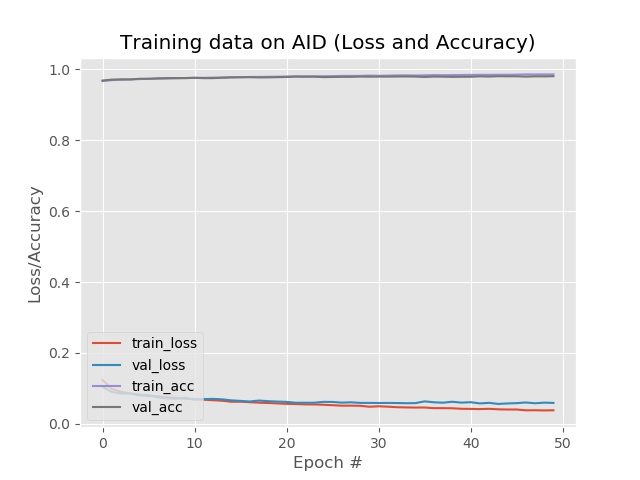
\includegraphics[scale=0.3]{ModelTrain.jpg}

Como é possível ver no gráfico acima, o sucesso do nosso modelo chega aos 98\%, sendo que as perdas são mínimas.

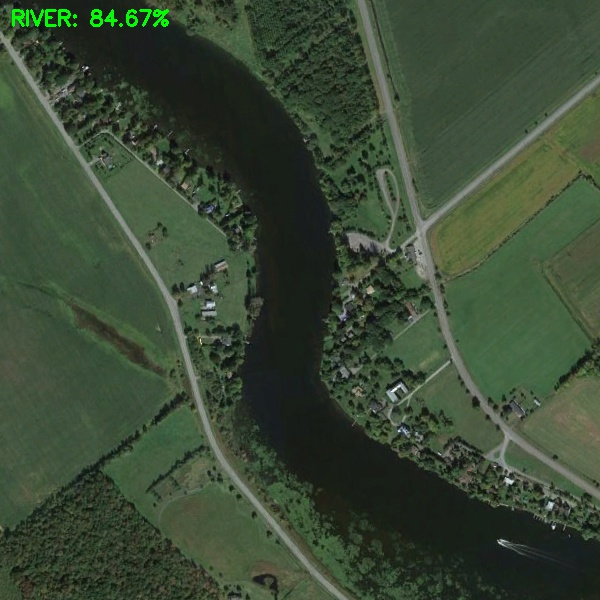
\includegraphics[scale=0.3]{Prediction.jpg}

A imagem acima representa um exemplo de um rio correctamente identificado com, aproximadamente, 84\% de certeza.

\section{Performance do sistema e situações de erro}

A performance de todo o sistema é satisfatória, desde o tempo que demora cada época de treino da inteligência artificial até às previsões correctas de cada imagem, dentro ou fora do conjunto de imagens testadas. \\
No entanto, é de notar que nem todas as imagens são etiquetadas correctamente (através da previsão utilizando o modelo). Isto deve-se à semelhança nos detalhes das diversas imagens existentes. Um caso possível que aconteceu durante testes, foi a etiquetagem pelo programa de uma estação de comboio como uma escola (são ambos edifícios relativamente grandes, usualmente no centro de áreas urbanas).

\section{Conclusão}

Na ciência da visão por computador, apesar de existirem diversas tecnologias diferentes para alcancar o mesmo objectivo, foi observado através do trabalho que nos foi proposto, que é definitivamente melhor utilizar tecnologias e algoritmos específicos para melhor alcançar resultados que se alinhem com o nosso objectivo. \\
Também se conseguiu através deste trabalho observar o quão poderosas são as ferramentas que utilizamos, e como as aplicar noutros cenários.

\nocite{*}
\bibliography{egbib}




%------------------------------------------------------------------------

\end{document}
